
These are activities to do every week. You will hand this sheet in at
the end of the semester. If we are outdoors in lab, fill in all pages.
If we are indoors during lab, just fill in the Moon section if there
is some clear night that week.

\noindent
{\bf Draw Polaris, Casseopia}  

Put Polaris at the center of this plot. Draw the ``W'' of Casseopia as
it appears each night in lab at around 7:30pm Standard Time. This will
be 8:30pm Daylight Time. Mark each location with a date.
 
\begin{minipage}[b]{8cm}{\psfig{figure={o3s_f1.eps},width=14.0cm}}\end{minipage}

%\clearpage
%
%\noindent
%{\bf Chart Mars throughout the semester}  
%
%Using the chart on the next page reproduced from the Sky \& Telescope
%Atlas, on every clear lab find Mars and place it as accurately as you
%can on this chart, with a point and a date.
%
%\clearpage
%
%\hspace{-0.3in} 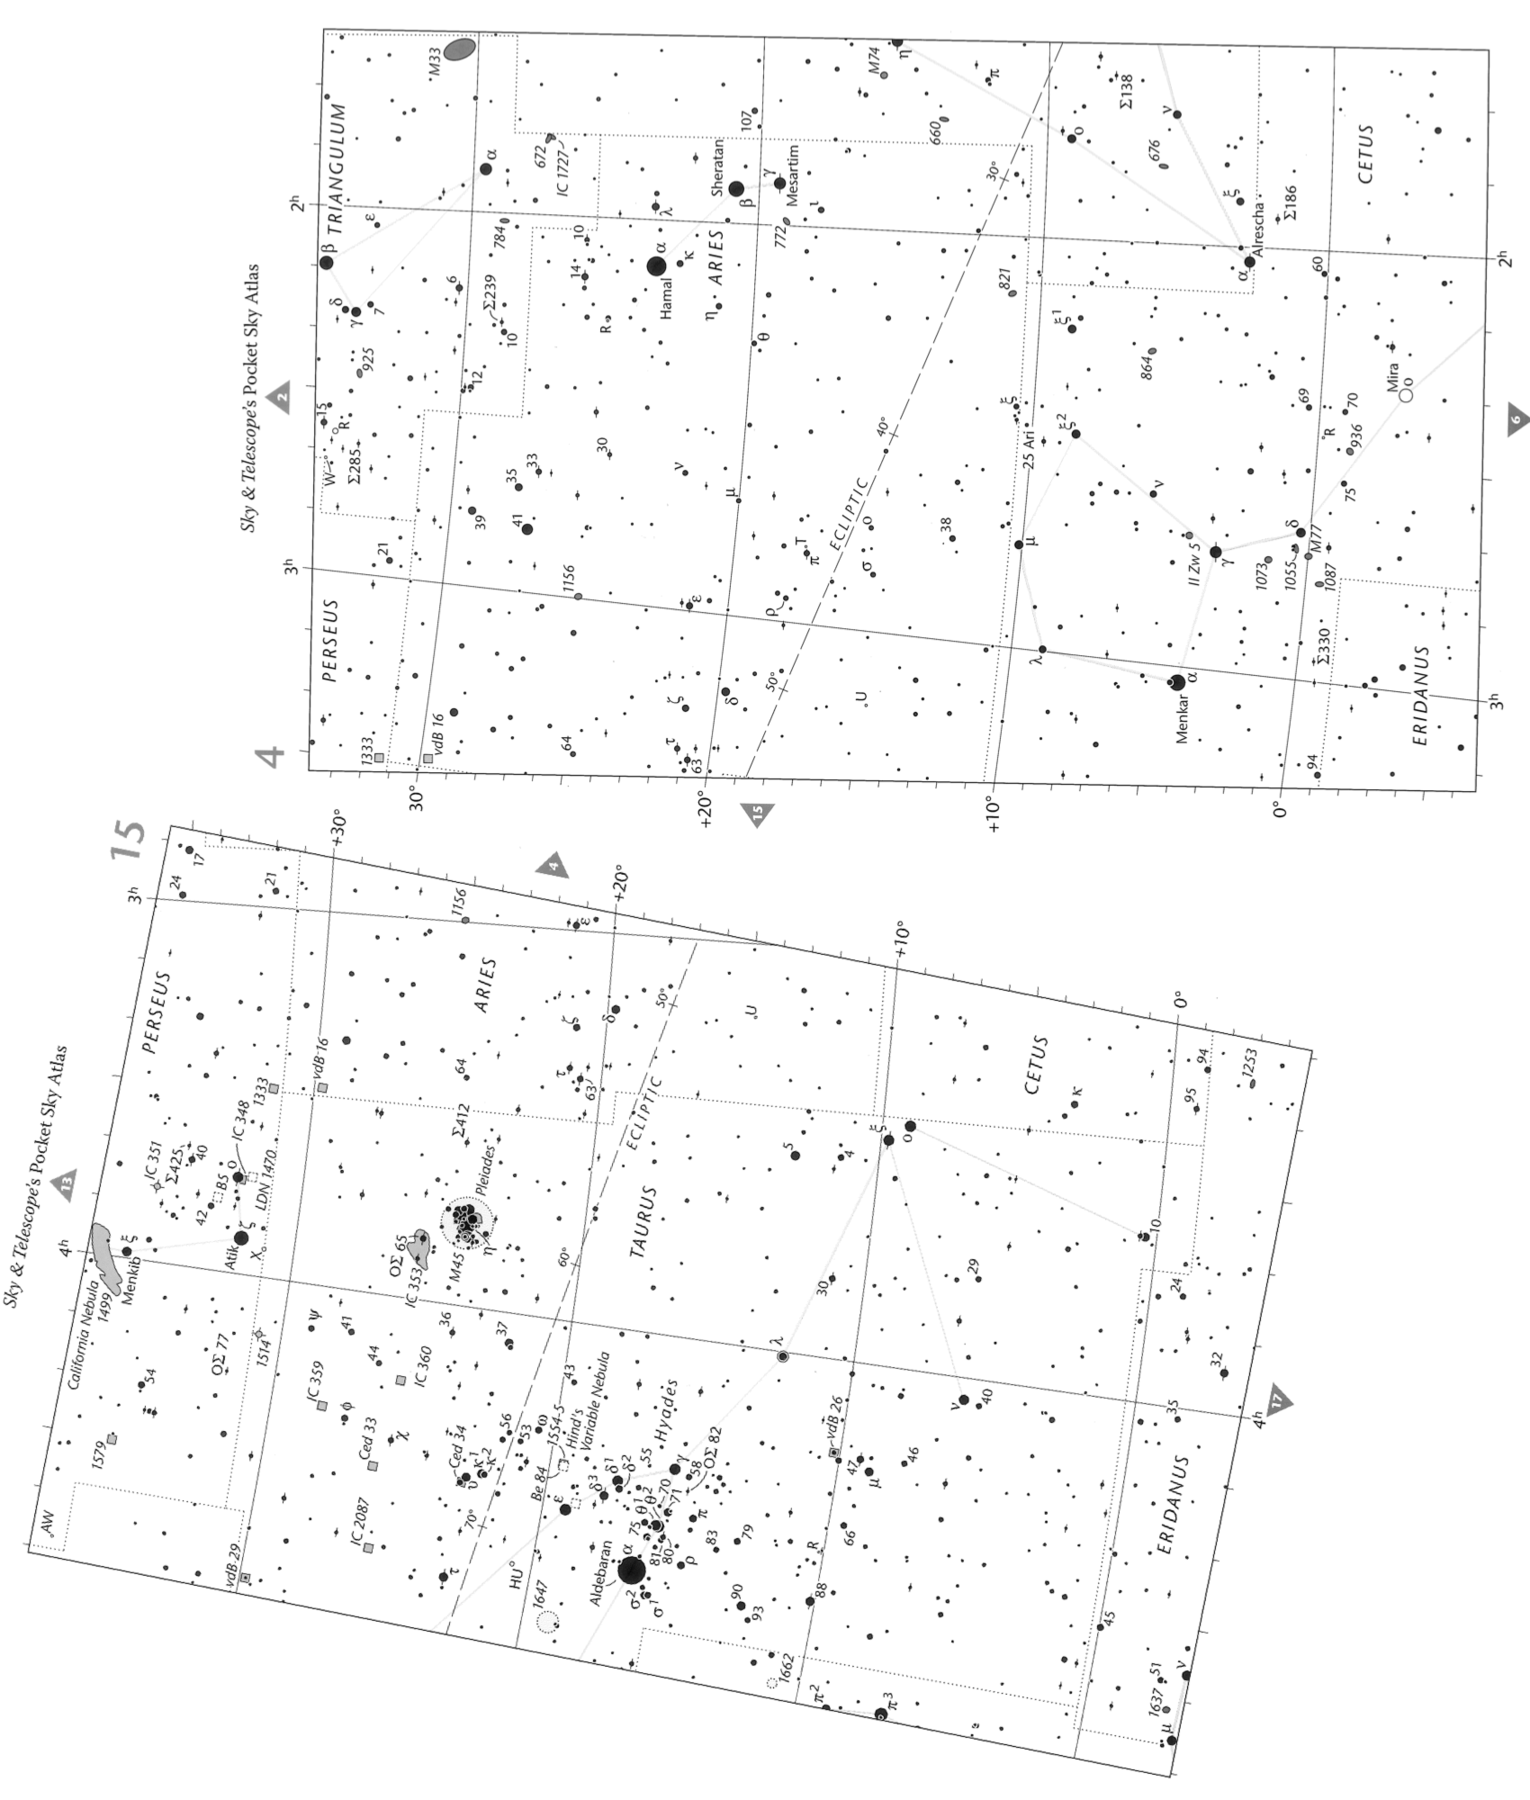
\includegraphics[width=7.5in]{mars-together.eps}

\clearpage

\noindent
{\bf Pay attention to the Moon}  

During lab, if we are outdoors, or sometime else in the week when the
weather is clear, look outside around 8pm and check if the Moon is
visible in the sky. Enter in the table below: (a) whether it is in the
East, West, or South; (b) what its phase is (full, new, crescent,
gibbous, and whether waxing or waning); and (c) guess what you will
find next week.

\begin{table}[h!]
\begin{tabular}{|c||c|c|c|}
\hline
{\bf Date} & {\bf Moon up at 8pm?} & {\bf Moon phase} & {\bf Guess for next
week} \cr
\hline
\hline
 & & & \cr
\hline
 & & & \cr
\hline
 & & & \cr
\hline
 & & & \cr
\hline
 & & & \cr
\hline
 & & & \cr
\hline
 & & & \cr
\hline
 & & & \cr
\hline
 & & & \cr
\hline
 & & & \cr
\hline
 & & & \cr
\hline
 & & & \cr
\hline
 & & & \cr
\hline
 & & & \cr
\hline
 & & & \cr
\hline
 & & & \cr
\hline
 & & & \cr
\hline
 & & & \cr
\hline
\end{tabular}
\end{table}
